\documentclass[11pt]{ctexart}

\usepackage{multicol}
%\usepackage{mwe}
\usepackage{subfigure}
\usepackage{mathtools}
\usepackage{graphicx}
\usepackage{amsmath}
\usepackage{mathrsfs}
\usepackage[top=0.5in,bottom=1in,left=1in,right=1in]{geometry}
\usepackage{pdflscape}
\usepackage{times}
\usepackage{bm}
%\usepackage{setspace}
\usepackage{color}
\usepackage{caption}
\usepackage{amsmath}
\usepackage{amssymb}
\usepackage{CJK}
%\usepackage[final]{pdfpages}
\usepackage{listings}
\usepackage{textcomp}
\usepackage{xcolor}
\usepackage{algorithm2e}
\usepackage{float}
\usepackage{algorithmicx}
\usepackage{algpseudocode}
\usepackage{hyperref}

\hypersetup{hidelinks,
	colorlinks=true,
	allcolors=black,
	pdfstartview=Fit,
	breaklinks=true}

\pagestyle{plain}




\begin{document}

\title{第四周实习报告20220322}
\author{宋欣源}
\date{\today}

\maketitle % need full-width title

\CTEXsetup[format={\Large\bfseries}]{section}

\section{第一,综述}

下面对于这些天实习的工作做一个报告。上周请了几天假,所以做的工作能写的不多,现在就两周的工作做一个总结
我这周主要分成两个大的方向,CNN和RNN

\section{第一,CNN}
\subsection{CNN2d}
在CNN领域,首先,继续上次的研究,利用CNN2d进行了一系列实验,将层数提高到三层,四层

模型1:普通CNN2d(ordinary*2+pointwise+linear*2+dropout+relu)

{\kaishu \small IC: 0.058, pnl:2.0}

~\\
模型2:普通CNN2d(deepwise*2+pointwise+linear*2+dropout+relu)

{\kaishu \small IC: 0.057, pnl:2.1}

~\\
模型3:普通CNN2d(ordinary*2+linear*2+pointwise+linear*2+dropout+relu)

{\kaishu \small IC: 0.048, pnl:1.9}

~\\
模型4:普通CNN2d(deepwise*2+linear*2+pointwise+linear*2+dropout+relu)

{\kaishu \small IC: 0.062, pnl:2.0}

~\\
模型5:普通CNN2d(deepwise*2+maxpool+linear*2+pointwise+linear*2+dropout+relu)

加入maxpool以后效果相对变差,但是对于巨大的模型,maxpool的效果往往是正向的。maxpool不能直接接着最后的时间序列提取,中间一定要有别的层作为过渡。

{\kaishu \small IC: 0.042, pnl:1.8}

~\\
模型6:普通CNN2d(deepwise*2+ordinary+linear*2+pointwise+linear*2+dropout+relu)

相当于三层特征CNN2d提取,一层时间序列注意力提取,目前没有出现训练epoche增多效果变差的情形,所以暂不考虑模型过大

{\kaishu \small IC: 0.066, pnl:2.2}

~\\
模型7:普通CNN2d(deepwise*2+ordinary*3+linear*2+pointwise+linear*2+dropout+relu)

相当于五层特征CNN2d提取,一层时间序列注意力提取,效果又有变化,但是在第四个epoche开始变差,过拟合信号比较危险。所以CNN2d在这个数据集上最适合的层数是4层特征。

{\kaishu \small IC: 0.068, pnl:2.4}

\subsection{CNN1d}
CNN1d的应用范围就非常广了,可以将时间序列当成一维音频数据,进行提取,也不用考虑过多的技巧。因此在一维CNN上设计了大量模型进行尝试。

模型1:普通CNN1d(ordinary*2+avg+linear*2+dropout+relu)

{\kaishu \small IC: 0.042, pnl:1.8}

~\\
模型2:普通CNN1d(ordinary*2+avg+ordinary*2+linear*2+dropout+relu)

{\kaishu \small IC: 0.045, pnl:1.9}

~\\
模型3:普通CNN1d(ordinary*2+avg+ordinary*2+linear*2+pointwise+dropout+relu)

{\kaishu \small IC: 0.052, pnl:1.9}

~\\
模型4:普通CNN1d((ordinary+avg+relu)*3+(ordinary+relu)*2+ordinary+linear*2+dropout+relu)

这个模型采用了三个largeFOV代码块,后面两次受限于序列长度不能再使用avgpool方法,largeFOV本身是用来做语义特征的提取,这里采用进行时间序列特征提取。提取之后的信息,不经过解码,而是用avgpool压缩到一个点上,用来代替时间序列在界面上的注意力。单独的largeFOV效果还不很好,进一步探索。结构如下图

\begin{figure}[H]
\begin{center}
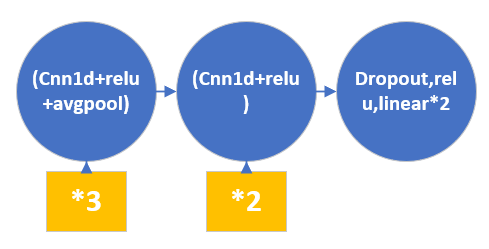
\includegraphics[width=0.5\textwidth]{str1.PNG}
\end{center}
\caption{model4 structure figure}
\label{FIG.1}
\end{figure}
{\kaishu \small IC: 0.052, pnl:1.8}

~\\
模型5:普通CNN1d((ordinary+avg+relu)*3+(ordinary+relu)*3+ordinary+linear*2+dropout+relu)

对于模型4,很容易想到的改进就是继续加层,不妨再加一个largeFOV代码块.为了保证效果不会变差,采用残差网络将原来的模型加上去,结构图如下图:
\begin{figure}[H]
\begin{center}
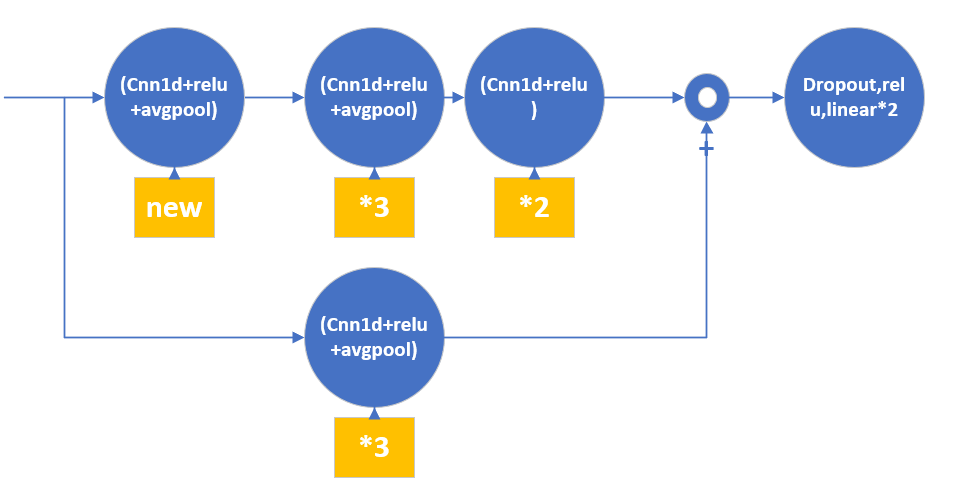
\includegraphics[width=0.8\textwidth]{str2.PNG}
\end{center}
\caption{model5 structure figure}
\label{FIG.2}
\end{figure}

{\kaishu \small IC: 0.050, pnl:2.0}

~\\
模型6:普通CNN1d((ordinary+avg+relu)*4+(ordinary+relu)*3+ordinary+linear*2+dropout+relu)

对于模型5,很容易想到的改进就是继续加层,不妨再加一个largeFOV代码块.为了保证效果不会变差,采用残差网络将原来的模型加上去,这一次,就是两个resnet代码块,这样保证效果至少不会比之前的效果差。同时需要注意,模型5的resnet也保留,但是由于输入输出已经修改了,所以要改成新的特征维度。结构图如下图:
\begin{figure}[H]
\begin{center}
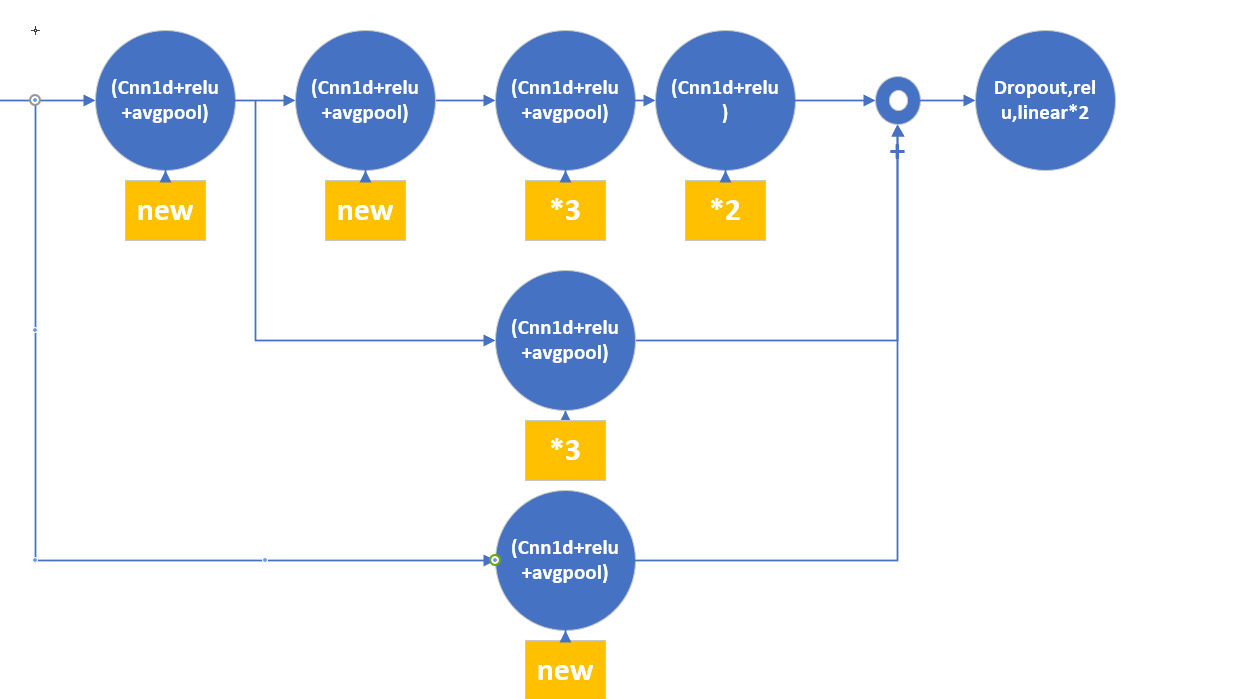
\includegraphics[width=0.8\textwidth]{str3.PNG}
\end{center}
\caption{model6 structure figure}
\label{FIG.3}
\end{figure}

{\kaishu \small IC: 0.050, pnl:2.1}

~\\
模型7:普通CNN1d((ordinary+avg+relu)*5+(ordinary+relu)*3+ordinary+linear*2+dropout+relu)

既然这个方法能有提高,那我就继续加层,同时保证结构结构,按这个方法制作三级模型。图如下图:
\begin{figure}[H]
\begin{center}
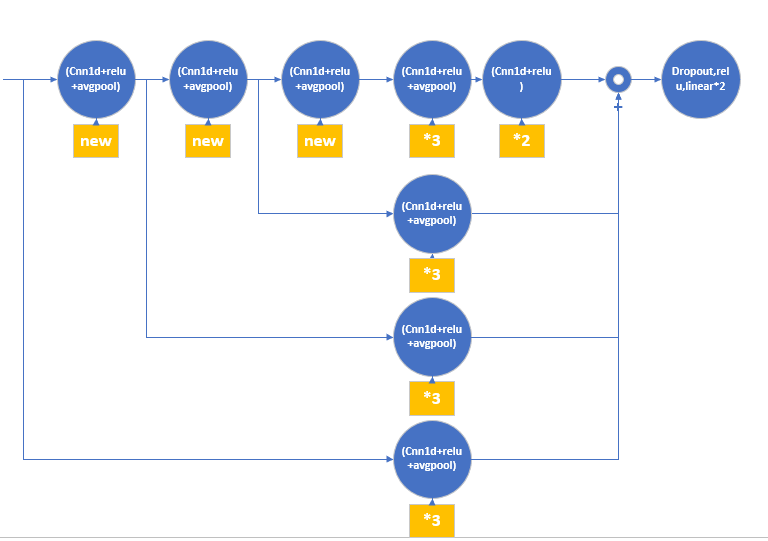
\includegraphics[width=0.8\textwidth]{str4.PNG}
\end{center}
\caption{model7 structure figure}
\label{FIG.4}
\end{figure}

{\kaishu \small IC: 0.061, pnl:2.25}

~\\
模型8:普通CNN1d((ordinary+avg+relu)*6+(ordinary+relu)*3+ordinary+linear*2+dropout+relu)

既然这个方法能有提高,那我就继续加层,同时保证结构结构,按这个方法制作三级模型。图如下图:
\begin{figure}[H]
\begin{center}
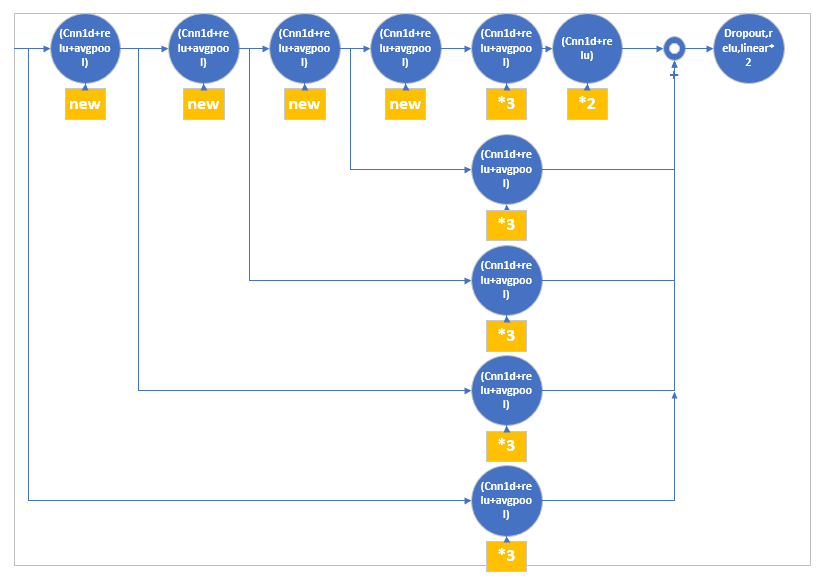
\includegraphics[width=0.8\textwidth]{str5.PNG}
\end{center}
\caption{model8 structure figure}
\label{FIG.5}
\end{figure}

{\kaishu \small IC: 0.070, pnl:2.42}

这个时候,受限制于时间序列的长度,我只取了40的长度,所以不能继续加层了,(每层都会有长度损失,如果使用padding,相当于人为添加了很多0,不可取)如果时间序列长度修改,模型就要大修,目前还没有继续做。

~\\
模型9:bottleneck((cnn1d(1)+cnn1d(3)+cnn1d(1))+pointwise+linear+dropout+relu)

模型9开始换一个提取思路,之前的所有cnn都采取v卷积核为3的ordinary卷积层,现在换成卷积核为1的卷积层。先升高维度,再进行特征提取,最后再用1维卷积核降低维度,提取特征以后,用pointwise做时间序列抽取。同时,为了保证结果有效性,加上一个普通的x输入作为残差神经网络。结构如图:
\begin{figure}[H]
\begin{center}
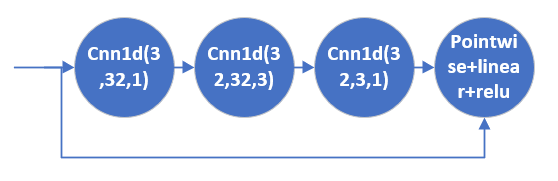
\includegraphics[width=0.5\textwidth]{str6.PNG}
\end{center}
\caption{model9 structure figure}
\label{FIG.6}
\end{figure}

{\kaishu \small IC: 0.060, pnl:1.7}

~\\
模型10:bottleneck((cnn1d(1)+cnn1d(3)+cnn1d(1))+pointwise+linear+dropout+relu)

模型10是另一种bottleneck,提取特征以后,用pointwise做时间序列抽取。同时,为了保证结果有效性,加上一个卷积层作为残差神经网络。模型9和模型10都是bottleneck模型的结构体,用来作为其他大型模型的小的分支。后面利用这两个结构进行研究。结构如图:
\begin{figure}[H]
\begin{center}
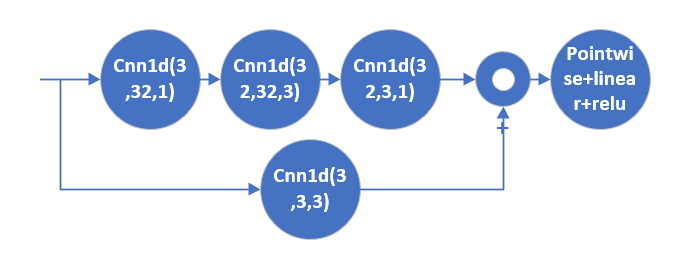
\includegraphics[width=0.7\textwidth]{str7.PNG}
\end{center}
\caption{model10 structure figure}
\label{FIG.7}
\end{figure}

{\kaishu \small IC: 0.059, pnl:1.7}

~\\
模型11:base((cnn1d+batchnorm+relu+avgpool)*2+pointwise+linear+dropout+relu)

模型11是接下来要做的模型的base,与之前不同的地方在于增加了batchnorm

{\kaishu \small IC: 0.031, pnl:1.4}

~\\
模型12: bottleneck((cnn1d+batchnorm+relu+avgpool)*2+bottleneck1+pointwise

+linear+dropout+relu)

模型12在和模型11做对比,加入了bottleneck1的层次。相当于对于卷积提取的信号,利用bottleneck1整理到自己想要的维度。效果还不是很好。

{\kaishu \small IC: 0.035, pnl:1.5}

~\\
模型13: bottleneck((cnn1d+batchnorm+relu+avgpool)*2+bottleneck2+pointwise

+linear+dropout+relu)

模型13在和模型11做对比,加入了bottleneck2的层次。相当于对于卷积提取的信号,利用bottleneck2整理到自己想要的维度。效果还不是很好。但是没有放弃这个思路,继续添加层次。

{\kaishu \small IC: 0.039, pnl:1.37}

~\\
模型14: bottleneck((cnn1d+batchnorm+relu+avgpool)*2+bottleneck1+bottleneck2+pointwise

+linear+dropout+relu)

模型14在和模型11做对比,加入了bottleneck1和bottleneck2的两个层次。相当于对于卷积提取的信号,利用两次bottleneck整理到自己想要的维度。这样做的意义在于利用bottleneck替换上面研究的largeFOV卷积结构,因为上面的结构都是五个六个largeFOV起步,但是我不确定bottleneck的效果怎么样,所以一个一个叠加。效果还不是很好。但是没有放弃这个思路,继续添加层次。

{\kaishu \small IC: 0.045, pnl:1.4}

~\\
模型15: deepnn((cnn1d+batchnorm+relu+avgpool)*2+bottleneck1

+bottleneck2+bottleneck1+bottleneck2+pointwise+linear+dropout+relu)

模型15在和模型11做对比,加入了两个bottleneck1和两个bottleneck2的两个层次。效果马上变好,比较正常,可以进行下一步研究。原因是bottleneck只是普通的卷积结构,其效果稍好于一层卷积结构,虽然参数增多了很多,但是不能改变一个算子带来的影响。算子越多,特征越清晰,但是过拟合风险越大。所以也没有继续添加bottleneck。结构图如下图:
\begin{figure}[H]
\begin{center}
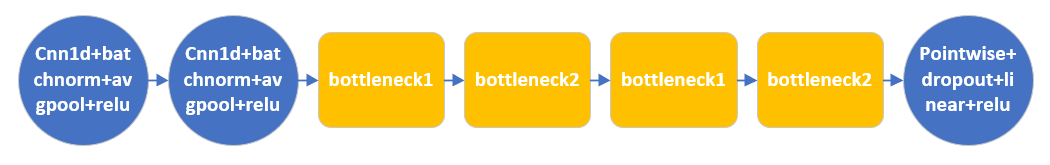
\includegraphics[width=0.8\textwidth]{str8.PNG}
\end{center}
\caption{model15 structure figure}
\label{FIG.8}
\end{figure}

{\kaishu \small IC: 0.068, pnl:2.0}

~\\
模型16: multigrid(base+multigrid+poitwise)

model16的结构是multigrid。multigrid的意思是利用多种不同的卷积方式进行卷积,最后把结果加在一起,这样一旦有哪个卷积模型让结果变得不好,就可以避免。同时多种卷积加在一起,提高了特征提取的鲁棒性,不会因为数据整体偏移而产生错误的结果。multigrid的方法图下图所示:
\begin{figure}[H]
\begin{center}
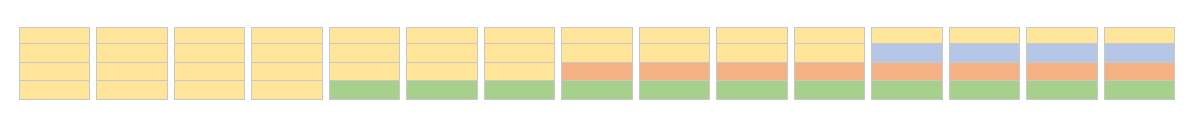
\includegraphics[width=0.9\textwidth]{str9.PNG}
\end{center}
\caption{其中,每个方块代表一个数据,蓝色表示卷积1的作用范围,黄色表示卷积2,红色表示卷积3,绿色表示卷积4,最后将四个卷积的结果加起来。}
\label{FIG.9}
\end{figure}
可以看到,不同的卷积在长度为16的序列里采用了不同的卷积方式,采用了不同的数据,非常类似于挖因子过程中,不同长度的滑动时间窗口的均线叠加在一起,这样增加了短期趋势的作用,同时提高了长期趋势的作用,减少了数据的过拟合。multigrid卷积出来的特征,同时增强了短期和长期特征,而且四种特征加起来,很好的提高了鲁棒性。在语义提取中,multigrid往往采用更复杂的膨胀卷积和缩合卷积完成,我下一步也用这两种卷积进行尝试。

有了multigrid以后,还需要将不同长度的卷积加起来,这里我采用了双线性插值,让数据的长度报保持一样。最后再用pointwise进行特征提取.结构图如下图:
\begin{figure}[H]
\begin{center}
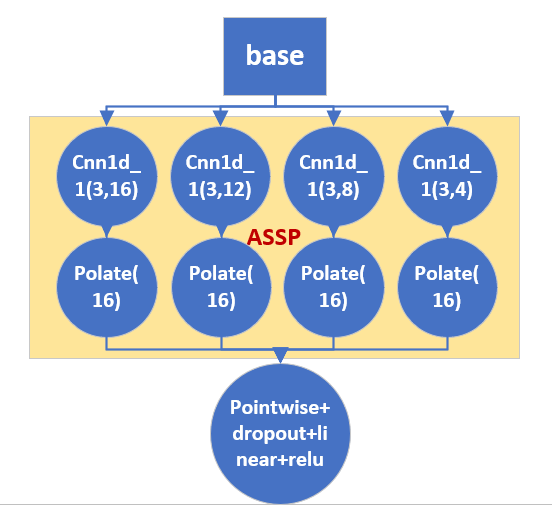
\includegraphics[width=0.6\textwidth]{str10.PNG}
\end{center}
\caption{multigrid和bilinearinterpolate模型16 structure figure}
\label{FIG.10}
\end{figure}
结果图:
\begin{figure}[H]
\begin{center}
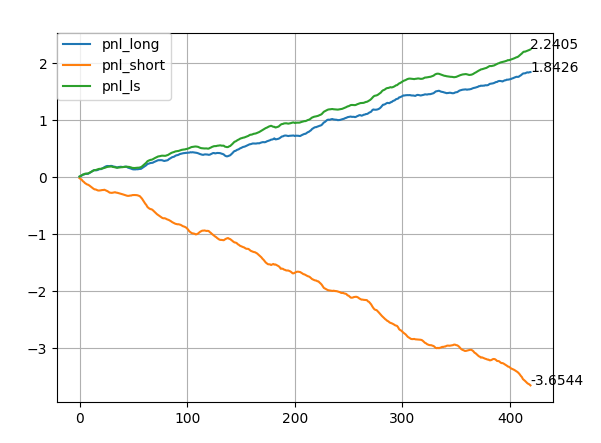
\includegraphics[width=0.8\textwidth]{plt1.PNG}
\end{center}
\caption{multigrid result figure}
\label{FIG.11}
\end{figure}

{\kaishu \small IC: 0.073, pnl:2.3}

效果还是上不去,非常郁闷,可能是插值的原因,下一步换个办法叠加数据。

~\\
模型17: multigrid+bottleneck(base+bottleneck+multigrid\_assp+linear)

模型17就是将bottleneck的成型版本和multigrid叠加起来,先进行bottleneck的特征提取,对于新的特征层,利用multigrid进行二次提取。结构图如下:
\begin{figure}[H]
\begin{center}
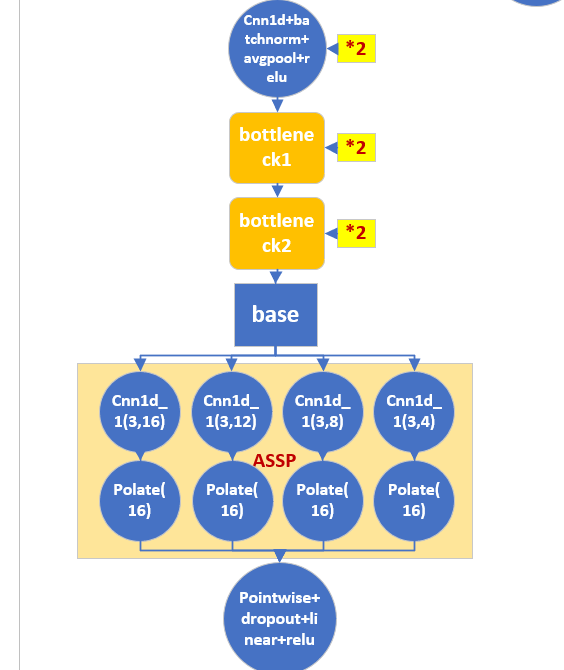
\includegraphics[width=0.7\textwidth]{str11.PNG}
\end{center}
\caption{multigrid和bottleneck模型17 structure figure}
\label{FIG.12}
\end{figure}

{\kaishu \small IC: 0.071, pnl:2.3}

~\\
模型18:multigrid+bottleneck(base+bottleneck+multigrid\_batchnorm+linear)

模型18就是将在模型17的基础上,把multigrid的每一个卷积都换成FOV,也就是加入batchnorm,avgpool,relu三个层次。接下来和17一样,先进行bottleneck的特征提取,对于新的特征层,利用multigrid进行二次提取。得到的结果IC有明显提高,但是pnl还是不改变,这个实验也侧面说明multigrid是有用的,可能是bottleneck的问题,为了验证这一步,不妨再在multigrid里加上resnet进行验证。

{\kaishu \small IC: 0.072, pnl:2.3}

~\\
模型19:multigrid+bottleneck(base+bottleneck+multigrid\_batchnorm+linear)

模型19就是将在模型18的基础上,在multigrid里加上resnet,resnet只做卷积核为1的卷积,同时做一个平均的操作,保证和其他的multigrid卷积结果数据长度一样,relu和batchnorm也保持一样。结构图如下如:
\begin{figure}[H]
\begin{center}
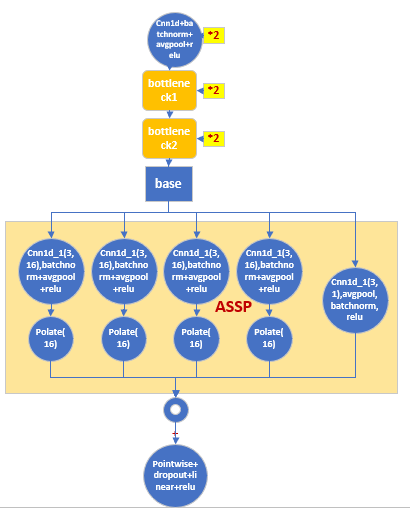
\includegraphics[width=0.8\textwidth]{str12.PNG}
\end{center}
\caption{multigrid和bottleneck resnet19 structure figure}
\label{FIG.13}
\end{figure}
计算出的结果还是一样。

{\kaishu \small IC: 0.072, pnl:2.3}

~\\
模型20:multigrid+bottleneck(base+bottleneck+multigrid\_batchnorm+linear)

模型20是暴力删去双线性插值,直接采取每个特征在时间序列上最后的1个数据作为时间序列,同时删去poitwise,poitwise已经验证是一个很好的办法,比提取最后一位数据要好,但是双线性插值的结果不可控,所以要想提高只能通过这个手段,下一步还要研究其他的插值方法,或者将数据对齐的办法,目前想到的办法有稀疏矩阵方法,计算相关性方法。

计算的结果不如上面,但是我觉得还是插值的问题。

{\kaishu \small IC: 0.068, pnl:2.1}

~\\
模型21:multigrid+bottleneck(base+bottleneck+multigrid\_batchnorm+downsample)

模型21是在模型19的基础上,用下采样代替linear线性层,线性层本身没啥用,下采样的结构很简单,就是用1维kernel1的卷积将升高的64个维度降低到10个维度,再用poitwise提取最后的特征。

{\kaishu \small IC: 0.064, pnl:2.1}

~\\
模型22:multigrid(multigrid\_batchnorm+downsample)

模型22是在想,到底multigrid有没有用呢,答案是肯定的,将base和bottleneck和poitwise和双线性插值都去掉,单独的multigrid模型,就是模型22,模型的结果有了一点提高,说明其他几个模型其实在脱multigrid的后退。具体的结果还要进一步研究。

{\kaishu \small IC: 0.070, pnl:2.45}

~\\
模型23:multigrid(multigrid\_batchnorm+downsample+upsample)

模型23有了这个结论,基于模型23进行新的卷积层的加入。在downsample后面再加一个卷积层,当作将已经降低的维度重新升高,再用poitwise进行特征提取。问题在于:为什么不在multigrid之前做卷积呢?答案是我们之前再multigrid前面做了大量的操作,结果都不理想,所以只能在后面添加卷积层。计算结果变差了,陷入了尴尬的情况。
模型结构如图:
\begin{figure}[H]
\begin{center}
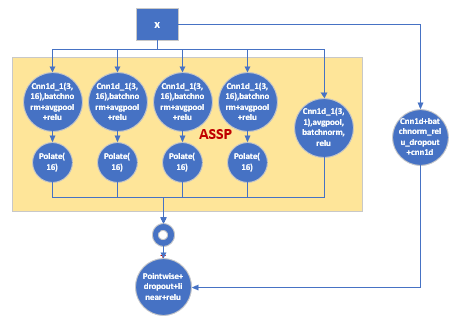
\includegraphics[width=0.8\textwidth]{str13.PNG}
\end{center}
\caption{multigrid23 structure figure}
\label{FIG.14}
\end{figure}

{\kaishu \small IC: 0.070, pnl:2.3}

~\\
模型24:multigrid(multigrid\_batchnorm+downsample+upsample)

模型24是总结模型。把我所用的所有方法:bottleneck1,bottleneck2,multigrid,双线性插值,downsample全都加在一起,利用resnet加以连接,模型结构图如图:
\begin{figure}[H]
\begin{center}
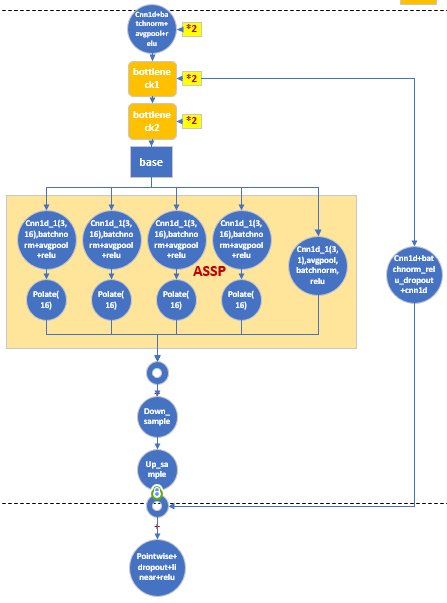
\includegraphics[width=0.8\textwidth]{str14.PNG}
\end{center}
\caption{final all model24 structure figure}
\label{FIG.15}
\end{figure}

{\kaishu \small IC: 0.068, pnl:2.25}

\subsection{改进思路}
\begin{itemize}
  \item [0)]
  设计了很多模型,进行了模型的堆叠,尽管效果一直上不去,受限于时间序列长度(只取了40)的原因,受限于水平还是不行。但是我觉得我模型设计能力提高了很多。收获颇丰。
  \item [1)]
  首先,对于CNN2d模型,尝试在特征提取方面已经有很多效果,所以下一步把注意力放在时间序列提取上,找代替pointwise的时间序列提取方法,比如instancewise,时间序列增强手术等方法,也可以用因子的方法在时间序列上做算符。
  \item [2)]
  对于CNN1d来讲,能操作的就太多了,可以从bottleneck,assp,FRC, multi-grid着手做模型拼接和模型演化,一点一点提高效果
\end{itemize}

\section{RNN的研究}
\subsection{综述}
RNN的研究主要是四个方面。研究cell和循环的写法,自创cell,在cell里运用多个时间节点,不同cell的串并联,以及其他复杂跨cell操作。

上周主要研究了cell的并联,这两周主要在研究cell的串联。

\subsection{cell串联}
构建好了各类的cell,就可以将cell进行串联,结构如下:
\begin{figure}[H]
\begin{center}
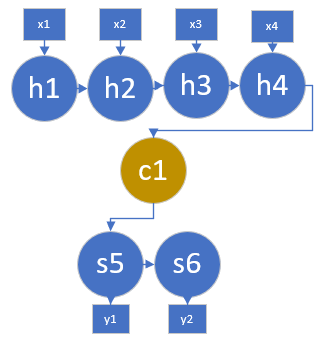
\includegraphics[width=0.5\textwidth]{series2.PNG}
\end{center}
\caption{cell的串联1 figure}
\label{FIG.16}
\end{figure}

也就是说,先通过一个RNNcell的循环,然后把cell state和hidden state保存下来,再用适当的方式进入下一个rnn cell。可以是hidden state本身作为新的hidden state,可以是hidden state经过数据变换作为新的hidden state,也可以是将之前所有state叠放在一起,经过变换变成新的state。
\begin{itemize}
  \item [1)]
  $h_{new} = h_n$
  \item [2)]
  $h_{new} = q(h_n)$
  \item [3)]
  $h_{new} = q(cat([h_1,h_2,h_3,h_4]))$

\end{itemize}

还有一种做法是将hidden state作为第二个cell每一步的输入,用公式表达就是
$$c_{<t>} = f(c_{<t-1>},x_t)$$
$$h_{<t>} = f(h_{<t-1>},y_{t-1},c)$$

因此,可以把串联1看成是串联2的简化
\begin{figure}[H]
\begin{center}
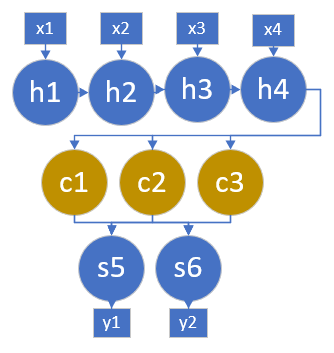
\includegraphics[width=0.5\textwidth]{series1.PNG}
\end{center}
\caption{cell串联2 figure}
\label{FIG.17}
\end{figure}

还有一种做法是如下图所示,用一个参数矩阵代表第一个cell的输出,然后每一个参数乘上矩阵的对应元素,得到新的输出,再用输出输入新的cell,用公式表达就是
$$h_{<t>} = f(W([h_{<t-1>},y_{t-1},c])+bias)$$

\begin{figure}[H]
\begin{center}
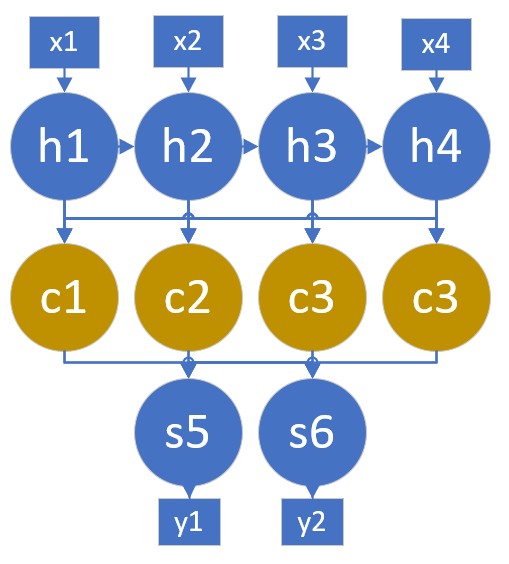
\includegraphics[width=0.5\textwidth]{series3.PNG}
\end{center}
\caption{cell串联3 figure}
\label{FIG.18}
\end{figure}

得到了以上三种串联结构以后,不妨设计以下几种类型:

\subsubsection{rnn1:串联加并联}
\begin{figure}[H]
\begin{center}
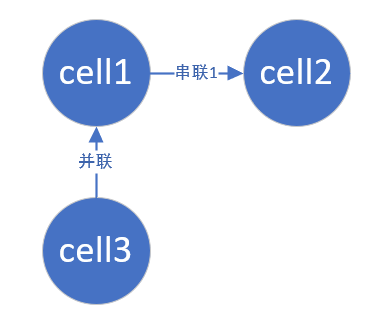
\includegraphics[width=0.5\textwidth]{rnn1.PNG}
\end{center}
\caption{串联加并联 figure}
\label{FIG.19}
\end{figure}
那么根据模型进行替换:
$$cell1 \rightrightarrows RNNcell, \quad cell2 \rightrightarrows RNNcell, \quad cell3 \rightrightarrows RNNcell$$

{\kaishu \small IC: 0.048, pnl:2.01}

$$cell1 \rightrightarrows LSTMcell, \quad cell2 \rightrightarrows LSTMcell, \quad cell3 \rightrightarrows LSTMcell$$

{\kaishu \small IC: 0.055, pnl:2.20}

\subsubsection{rnn2:(串联加并联)*2}
\begin{figure}[H]
\begin{center}
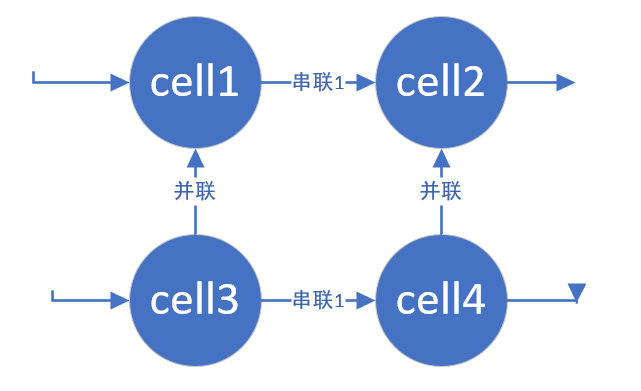
\includegraphics[width=0.5\textwidth]{rnn2.PNG}
\end{center}
\caption{(串联加并联)*2 figure}
\label{FIG.20}
\end{figure}
那么根据模型进行替换:
$$cell1 \rightrightarrows RNNcell, \quad cell2 \rightrightarrows RNNcell, \quad cell3 \rightrightarrows RNNcell, \quad cell4 \rightrightarrows RNNcell$$

{\kaishu \small IC: 0.058, pnl:2.21}

\begin{figure}[H]
\begin{center}
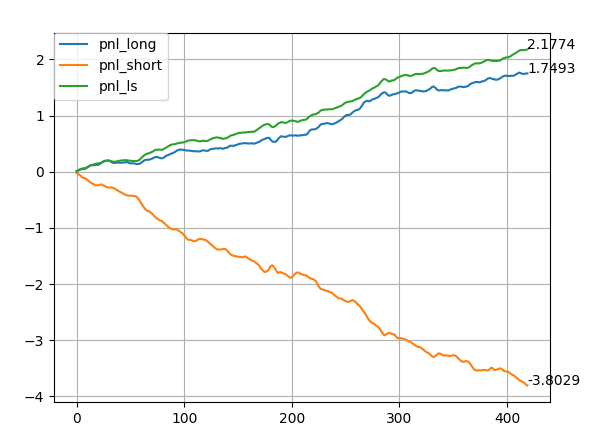
\includegraphics[width=0.8\textwidth]{plt2.PNG}
\end{center}
\caption{rnn result figure}
\label{FIG.21}
\end{figure}

$$cell1 \rightrightarrows GRUcell, \quad cell2 \rightrightarrows GRUcell, \quad cell3 \rightrightarrows GRUcell, \quad cell4 \rightrightarrows GRUcell$$

{\kaishu \small IC: 0.061, pnl:2.32} 

问题在于,为什么不能向上面一样利用lstm进行操作呢。
$$cell1 \rightrightarrows LSTMcell, \quad cell2 \rightrightarrows LSTMcell, \quad cell3 \rightrightarrows LSTMcell, \quad cell4 \rightrightarrows LSTMcell$$

发生了梯度消失,原因在于,把前一个lstm的cell state当作输入,cell state是用遗忘门和记忆门两个部分加起来组成的,那就会和自己本身的cell state的阶数不一样,经过cell2的循环以后,两者差距迅速拉大,其中一方远超过另一方,所以,在对cell2遗忘门的求导过程中,其中一部分造成了梯度消失。如果使用串联2的方法,效果是一样的,因为还是把cell state当作了新的输入。如果使用串联3的方法,效果不一样,目前串联三还没实现。

\subsubsection{rnn3:(串联加并联)+串联2}
问题在于,问什么不能在第二个串联处使用串联1呢,答案就是,立即发生梯度消失。对于cell2来说,只有把cell3的cell state全部输出到cell2之中,如果只是开头使用了输入, 那cell3和cell1的cell state肯定阶数不相等,立即发生梯度消失。如果cell2使用relu作为激活函数,立即发生梯度爆炸。

\begin{figure}[H]
\begin{center}
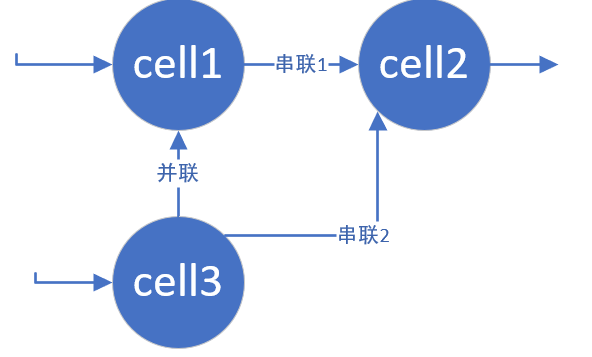
\includegraphics[width=0.5\textwidth]{rnn3.PNG}
\end{center}
\caption{(串联加并联)+串联2 figure}
\label{FIG.22}
\end{figure}
那么根据模型进行替换:
$$cell1 \rightrightarrows RNNcell, \quad cell2 \rightrightarrows RNNcell, \quad cell3 \rightrightarrows RNNcell$$

{\kaishu \small IC: 0.050, pnl:1.9}

$$cell1 \rightrightarrows GRUcell, \quad cell2 \rightrightarrows GRUcell, \quad cell3 \rightrightarrows GRUcell$$

{\kaishu \small IC: 0.059, pnl:2.2}

问题在于,为什么不能向上面一样利用lstm进行操作呢。
$$cell1 \rightrightarrows LSTMcell, \quad cell2 \rightrightarrows LSTMcell, \quad cell3 \rightrightarrows LSTMcell$$

发生了梯度消失。

\subsubsection{rnn4:(串联加串联联加串联}

\begin{figure}[H]
\begin{center}
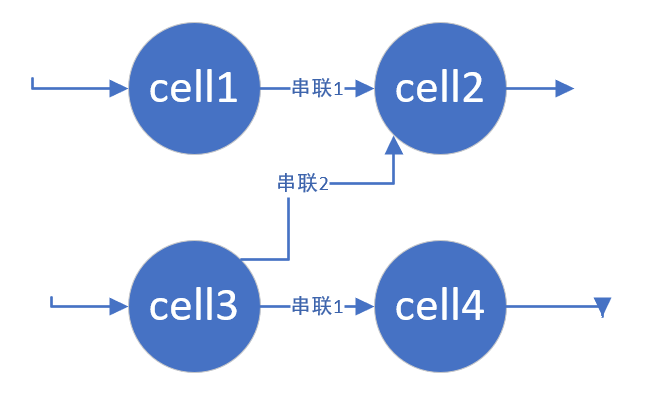
\includegraphics[width=0.5\textwidth]{rnn4.PNG}
\end{center}
\caption{串联加串联加串联 figure}
\label{FIG.23}
\end{figure}
那么根据模型进行替换:
$$cell1 \rightrightarrows RNNcell, \quad cell2 \rightrightarrows RNNcell, \quad cell3 \rightrightarrows RNNcell, \quad cell4 \rightrightarrows RNNcell$$

{\kaishu \small IC: 0.058, pnl:2.0}

$$cell1 \rightrightarrows GRUcell, \quad cell2 \rightrightarrows GRUcell, \quad cell3 \rightrightarrows GRUcell, \quad cell4 \rightrightarrows GRUcell$$

{\kaishu \small IC: 0.061, pnl:2.0}

下一步试一试将cell全都赋值为lstmcell进行试验

\subsubsection{rnn5:多个cell循环训练,其中两个作为输入输出}
这个模型的想法是,多个cell循环往复的训练,其效果肯定是越来越好的,越来越过拟合的,其中每次都随机挑两个cell输入输出,每次输入,肯定会让拟合度下降,抗过拟合度上升,训练的循环次数增加,拟合度上升,过拟合度上升。随即找两个就可以找到这两个点的平衡。代码上还有个核心问题,下一步思考解决。
\begin{figure}[H]
\begin{center}
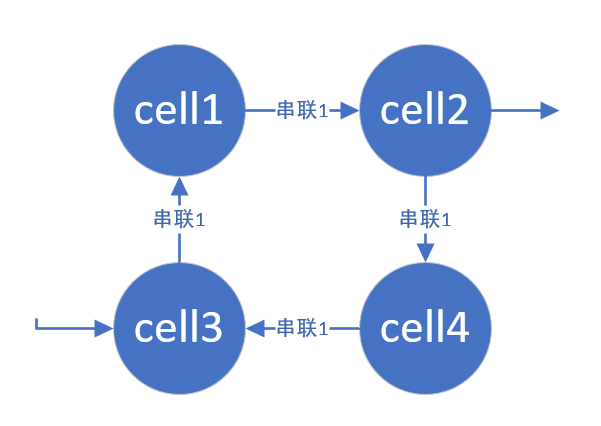
\includegraphics[width=0.5\textwidth]{rnn5.PNG}
\end{center}
\caption{多个cell循环训练,其中两个作为输入输出 figure}
\label{FIG.24}
\end{figure}


问题在于,以上做了这些cell的串并联,意义是否明显呢。意义并不明显。什么样的串并联意义明显呢,答案是,串并联的作用在于,将hidden state, output state,cell state和输出x都进行一定的操作和准备,每个数据都先经过一个模型训练过,然后再带入最后的简单的rnn网络训练,把这些工作总结起来,就是相当于四个rnncell连接在一起。这样就可以避免初始的各个state从0开始训练,影响最终效果的情况。究竟什么样的cell能起到数据先行训练的效果,目前手中的cell肯定不行,还需要设计新的特定功能的cell.所以下一步rnn的研究方向是,先利用最简单的数据进行预处理,再用最简单的cell完成训练。

\subsubsection{rnn6:并联预训练,并联实际训练}
基于上述想法,首先做了这个尝试
\begin{figure}[H]
\begin{center}
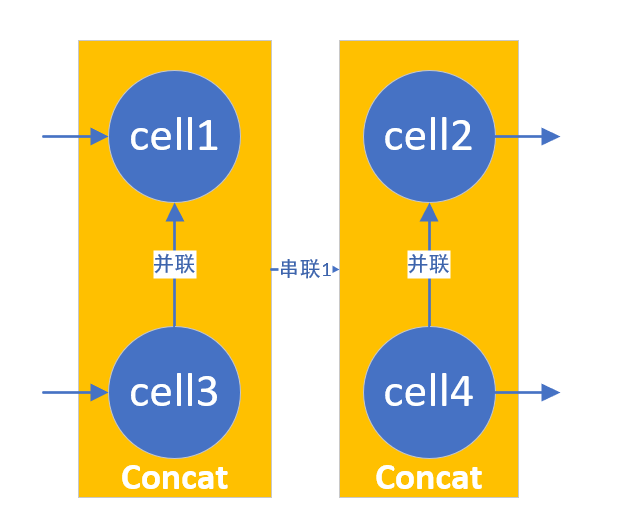
\includegraphics[width=0.5\textwidth]{rnn6.PNG}
\end{center}
\caption{并联预训练,并联实际训练 figure}
\label{FIG.25}
\end{figure}
cell1和cell3一起训练,训练完取平均,带入cell2和cell4训练完再取平均。
$$cell1 \rightrightarrows RNNcell, \quad cell2 \rightrightarrows RNNcell, \quad cell3 \rightrightarrows RNNcell$$

{\kaishu \small IC: 0.050, pnl:2.1}

$$cell1 \rightrightarrows GRUcell, \quad cell2 \rightrightarrows GRUcell, \quad cell3 \rightrightarrows GRUcell$$

{\kaishu \small IC: 0.061, pnl:2.4}


\section{总结}
\begin{itemize}
  \item [1)]
  第一,对于CNN2d模型,尝试在特征提取方面已经有很多效果,所以下一步把注意力放在时间序列提取上,找代替pointwise的时间序列提取方法,比如instancewise,时间序列增强手术等方法,也可以用因子的方法在时间序列上做算符。
  \item [2)]
  第二,对于CNN1d来讲,能操作的就太多了,可以从bottleneck,assp,FRC, multi-grid着手做模型拼接和模型演化,一点一点提高效果
  \item [3)]
  第三,在RNN领域,自己再设计一些有用的cell,不仅仅用现有的10个cell
  \item [4)]
  第四,继续进行RNN的串并联研究,衍生出更复杂的串并联模块,适当增长学习时间序列,保证参数有更好的发挥空间,解决RNNcell的跨越,重叠,条件连接等内容。RNNcell代码比较难写,写出来由于各类图论可能最终结果是一样的,还有梯度消失和梯度爆炸的风险,还要加把劲研究。
  \item [5)]
  第五,做了这么多,感觉方向不对,我打算重新实验一些最简单的东西,比如只用股价,时间周期扩充到98个bar,还有模型精简化进行尝试,多用一些数据操作的技巧,减少对于深度学习传统方法的依赖,像挖因子一样先操作好数据,再用简单的cnn1d,lstm等模型进行训练试一试。模型不一定越复杂越有效。
  \item [6)]
  第六,这几天上海疫情,和二位老师的沟通也减少了,但是我们这边没事,我的研究没有落下,一直按照计划再做,一点一点提高。收到了一些condition offer,还得花时间再考托福练口语,希望不会对研究造成影响。

\end{itemize}


\end{document} 